% ch04-interpretation-domain.tex — Interpretation I = (Δ^I, ·^I)
% Shows domain elements, class extensions as subsets, individual denotations.
% Pedagogical purpose: make syntax→interpretation→denotation visually concrete.
\documentclass[tikz,border=5pt]{standalone}
\usepackage{fontspec}
\setmainfont{Times New Roman}
\usepackage{unicode-math}
\setmathfont{Cambria Math}
\usetikzlibrary{shapes.geometric,positioning,fit,backgrounds,arrows.meta}

\begin{document}
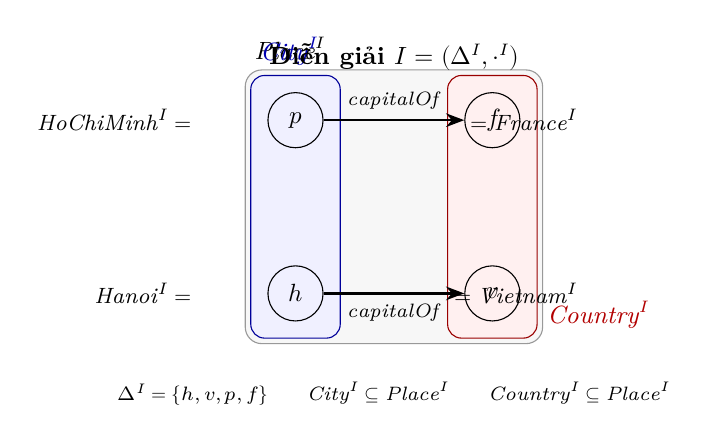
\begin{tikzpicture}[
  domainnode/.style={circle,draw,minimum size=0.7cm,inner sep=1pt,font=\small},
  classlabel/.style={font=\small\itshape,anchor=south west},
  indlabel/.style={font=\footnotesize,anchor=east},
  subsetline/.style={dashed,gray,line width=0.5pt},
  maparrow/.style={->,>=Stealth,thin,gray!70},
]

% Domain Δ^I
\node[domainnode] (h) at (0,0) {$h$};
\node[domainnode] (v) at (2.5,0) {$v$};
\node[domainnode] (p) at (0,2.2) {$p$};
\node[domainnode] (f) at (2.5,2.2) {$f$};

% Class extensions as rounded rectangles
\begin{scope}[on background layer]
  % Place^I = {h,v,p,f} — entire domain
  \node[fit=(h)(v)(p)(f), inner sep=8pt, draw=black!40, rounded corners=6pt,
        fill=black!3, label={[classlabel]north west:$\mathit{Place}^I$}] (place) {};

  % City^I = {h,p}
  \node[fit=(h)(p), inner sep=6pt, draw=blue!60!black, rounded corners=5pt,
        fill=blue!6, label={[classlabel,text=blue!70!black]north west:$\mathit{City}^I$}] (city) {};

  % Country^I = {v,f}
  \node[fit=(v)(f), inner sep=6pt, draw=red!60!black, rounded corners=5pt,
        fill=red!6, label={[classlabel,text=red!70!black]south east:$\mathit{Country}^I$}] (country) {};
\end{scope}

% Individual denotations (syntax → domain)
\node[indlabel] at (-1.2,0) {$\mathit{Hanoi}^I =$};
\node[indlabel] at (-1.2,2.2) {$\mathit{HoChiMinh}^I =$};
\node[indlabel] at (3.7,0) {$= \mathit{Vietnam}^I$};
\node[indlabel] at (3.7,2.2) {$= \mathit{France}^I$};

% capitalOf relation arrows
\draw[->,>=Stealth,thick] (h) -- node[midway,below,font=\scriptsize]{$\mathit{capitalOf}$} (v);
\draw[->,>=Stealth,thick] (p) -- node[midway,above,font=\scriptsize]{$\mathit{capitalOf}$} (f);

% Title
\node[font=\small\bfseries,anchor=north] at (1.25,3.3)
  {Diễn giải $I = (\Delta^I, {\cdot}^I)$};
\node[font=\scriptsize,anchor=north] at (1.25,-1.0)
  {$\Delta^I = \{h, v, p, f\} \qquad \mathit{City}^I \subseteq \mathit{Place}^I \qquad \mathit{Country}^I \subseteq \mathit{Place}^I$};

\end{tikzpicture}
\end{document}
